\documentclass[11pt, a4paper]{article}
\usepackage[a4paper, margin=1in]{geometry}

\usepackage{adjustbox}
\usepackage{mathtools}
\usepackage{amsmath}
\usepackage{amssymb}
\usepackage{amsthm}

\usepackage{pgfplots}
\usepackage{listings}
\usepackage{color}
\usepackage{tikz}

\usepackage{textcomp}
\usepackage{soul}

\usepackage[hidelinks]{hyperref}
\pgfplotsset{width=7.5cm,compat=1.12}
\usepgfplotslibrary{fillbetween}
\pgfplotsset{compat=1.8}
\usepgfplotslibrary{statistics}
\usepackage[makeroom]{cancel}
\title{\bf{Homework \textnumero 12}}
\author{Author: David Oniani
\\
\ \ \ Instructor: Dr. Eric Westlund}
\date{March 25, 2019}

\usepackage{listings}
\usepackage{color}

%%%%%%%%%%%%%%% S E T S %%%%%%%%%%%%%%%
\newcommand{\nats}{\mathbb{N}}
\newcommand{\ints}{\mathbb{Z}}
\newcommand{\rats}{\mathbb{Q}}
\newcommand{\reals}{\mathbb{R}}
\newcommand{\irrats}{\mathbb{I}}

\newcommand{\pnats}{\mathbb{N}^+}
\newcommand{\pints}{\mathbb{Z}^+}
\newcommand{\prats}{\mathbb{Q}^+}
\newcommand{\preals}{\mathbb{R}^+}
\newcommand{\nreals}{\mathbb{R}^-}

\newcommand{\nints}{\mathbb{Z}^-}
\newcommand{\nrats}{\mathbb{Q}^-}
%%%%%%%%%%%%%%%%%%%%%%%%%%%%%%%%%%%%%%%

% Calligraphy
\newcommand\und[1]{\underline{\smash{#1}}}

% Operators
\DeclarePairedDelimiter\abs{\lvert}{\rvert}
\DeclarePairedDelimiter\ceil{\lceil}{\rceil}
\DeclarePairedDelimiter\floor{\lfloor}{\rfloor}

% Other
\newcommand{\rarr}{\rightarrow}

\definecolor{dkgreen}{rgb}{0,0.6,0}
\definecolor{gray}{rgb}{0.5,0.5,0.5}
\definecolor{mauve}{rgb}{0.58,0,0.82}
\definecolor{backcolour}{rgb}{0.95,0.95,0.92}

\lstset{
backgroundcolor=\color{backcolour},
aboveskip=3mm,
belowskip=3mm,
showstringspaces=false,
columns=flexible,
basicstyle={\small\ttfamily},
numbers=left,
numberstyle=\normalsize\color{gray},
keywordstyle=\color{blue},
commentstyle=\color{dkgreen},
stringstyle=\color{mauve},
breaklines=true,
breakatwhitespace=true,
tabsize=4
}


\begin{document}
\maketitle
\begin{itemize}
\item[17.1]
\begin{itemize}
\item[(a)]
Since the sample size is 30, it is sufficient to say that the sampling
distribution of the sample mean is normal with the sample mean $\overline{x} = \mu = 50$
and the standard deviation $\frac{\sigma}{\sqrt{n}} = \frac{15}{\sqrt{225}} = 1.$
Below is the sketch that shows that 50 is the standard deviation, and 51, 52, and 53 are
points for 1, 2, and 3 standard deviations respectively.
\item[]
\item[]
\item[]
\begin{center}
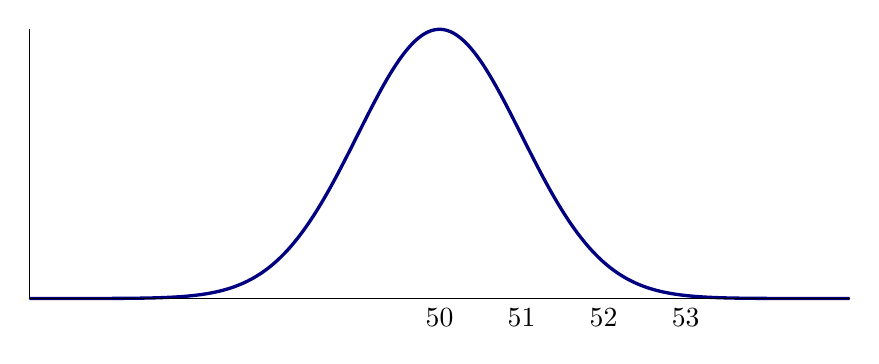
\begin{tikzpicture}
    \pgfmathdeclarefunction{gauss}{2}{%
    \pgfmathparse{1/(#2*sqrt(2*pi))*exp(-((x-#1)^2)/(2*#2^2))}%
    }
    \begin{axis}[
      no markers, domain=-5:5, samples=1000,
      axis lines*=left,
      height=5cm, width=12cm,
      xtick=\empty, ytick=\empty,
      enlargelimits=false, clip=false, axis on top,
      grid = major
      ]
      \addplot [very thick, blue!50!black] {gauss(0,1)};
      \node [below] at (500, 0) {$50$};
      \node [below] at (600, 0) {$51$};
      \node [below] at (700, 0) {$52$};
      \node [below] at (800, 0) {$53$};
    \end{axis}
\end{tikzpicture}
\end{center}

\item[]

\item[]

\item[(b)]
The result is towards the lower tail of the curve and point 48.9
is close to the center. Since $\mu = 50$, value like 48.9 would
not be a good evidence as it is really close to 50. On the other hand,
value 47.4 is too low as it is almost within 2 standard deviation from the mean.
It therefore provides a better evidence that $\mu < 50$. Below is the sketch.
\item[]
\item[]
\begin{center}
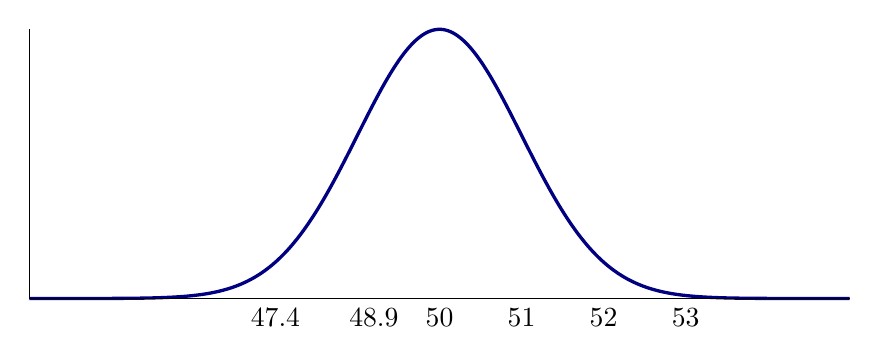
\begin{tikzpicture}
    \pgfmathdeclarefunction{gauss}{2}{%
    \pgfmathparse{1/(#2*sqrt(2*pi))*exp(-((x-#1)^2)/(2*#2^2))}%
    }
    \begin{axis}[
      no markers, domain=-5:5, samples=1000,
      axis lines*=left,
      height=5cm, width=12cm,
      xtick=\empty, ytick=\empty,
      enlargelimits=false, clip=false, axis on top,
      grid = major
      ]
      \addplot [very thick, blue!50!black] {gauss(0,1)};
      \node [below] at (300, 0) {$47.4$};
      \node [below] at (420, 0) {$48.9$};
      \node [below] at (500, 0) {$50$};
      \node [below] at (600, 0) {$51$};
      \node [below] at (700, 0) {$52$};
      \node [below] at (800, 0) {$53$};
    \end{axis}
\end{tikzpicture}
\end{center}
\end{itemize}

\item[]
\item[]

\item[17.3]
$H_0: \ \mu =  50$. $H_a: \ \mu < 50$.\\
$H_a: \ \mu < 50$ because the teacher think that poor attitudes are partly caused by the decline in scores.

\newpage

\item[17.11]
\begin{itemize}
\item[(a)]
$z = \displaystyle\dfrac{\overline{x} - \mu}{\sigma/\sqrt{}n} = \displaystyle\dfrac{48.9 - 50}{15/\sqrt{225}} \approx -1.10$.\\
Now, using Table A, we get that $P(z < -1.10) = 0.1357$. Since $P(z < -1.10) = 0.1357 > 0.05 > 0.01$,
it is not statistically significant at either $\alpha = 0.05$ or $\alpha = 0.01$.

\item[]

\item[(b)]
$z = \displaystyle\dfrac{\overline{x} - \mu}{\sigma/\sqrt{}n} = \displaystyle\dfrac{47.4 - 50}{15/\sqrt{225}} \approx -2.60$.\\
Now, using Table A, we get that $P(z < -2.60) = 0.0047$. Since $P(z < -1.10) = 0.0047 < 0.01 < 0.05$,
it is statistically significant at both $\alpha = 0.05$ or $\alpha = 0.01$.

\item[]

\item[(c)]
Outcomes tell us that $\overline{x} = 47.3$ is the strong evidence against
the null hypothesis since the $P$-value is 0.0047 which is really close to 0.
\\\\
Outcomes tell us that $\overline{x} = 48.9$ is not the strong evidence against
the null hypothesis since the $P$-value is 0.1357 which is not too close to 0.
\end{itemize}

\item[]
\item[]

\item[17.14]
We start with the STATE part.\\\\
\und{\textbf{STATE}}\\\\
$H_0: \ \mu = 10.1$ and $H_a: \ \mu \neq 10.1$
\\\\\\
\und{\textbf{SOLVE}}\\\\
$\overline{x} = \dfrac{10.08 + 9.89 + 10.05 + 10.16 + 10.21 + 10.11}{6} \approx 10.0833$.\\
$z = \displaystyle\dfrac{\overline{x} - \mu}{\sigma/\sqrt{}n} = \displaystyle\dfrac{10.0833 - 10.1}{0.1/\sqrt{6}} \approx -0.41$.\\
$P(z < -0.41 \text{ or } z > 0.41) = 2 \times P(z > 0.41) = 2 \times 0.3409 = 0.6818$.
\\\\\\
\und{\textbf{CONCLUDE}}\\\\
Since $P(z < -0.41 \text{ or } z > 0.41) = 0.6818 > 0.5$, there is not a sufficient evidence
that the true conductivity is not 10.1 (aka fail to reject $H_0$).

\item[]
\item[]

\item[17.16]
Notice that $z \approx 1.88$. Then $P(z > 1.88) = P(z < -1.88) = 0.0301$.\\
For $\alpha = 0.05$, $P < \alpha$ and therefore, is statistically significant.\\
For $\alpha = 0.01$, $P > \alpha$ and therefore, is not statistically significant.

\item[]
\item[]

\item[17.17]
Notice that $z \approx 1.88$. Then $P(z > 1.88 \text{ or } z < -1.88) = P(z < -1.88) = 2 \times 0.0301 - 0.0602$.\\
For $\alpha = 0.05$, $P > \alpha$ and therefore, is not statistically significant.\\
For $\alpha = 0.01$, $P > \alpha$ and therefore, is not statistically significant.

\item[17.30]
\begin{itemize}
\item[(a)]
The null hypothesis says that the population mean is equal to 15.
$H_0: \ \mu = 15$.

\item[]

\item[(b)]
$z = \displaystyle\dfrac{\overline{x} - \mu}{\sigma/\sqrt{}n} = \displaystyle\dfrac{15.3 - 15}{8.5/\sqrt{463}} \approx 0.76$.

\item[]

\item[(c)]
The $P$-value is $P(z > 0.76) = P(z < -0.76) = 0.2236$.
Now, since $P(z > 0.76) = 0.2236 > 0.05$, there is not
a strong evidence that the students study more than
15 hours per week on average.
\end{itemize}

\item[]
\item[]

\item[17.33]
The $P$-value is the probability that the test statistic
would take a value as or more extreme than observerd, assuming
$H_0$ is true, by chance error alone.\\\\
The student is wrong as the $P$-value is not the probability
of null hypothesis being true.

\item[]
\item[]

\item[17.44]
\begin{itemize}
\item[(a)]
$z_{\alpha/2} = z_{0.05} = 1.645$.\\
Then, the confidence interval is $\overline{x} \pm z_{\alpha/2} \times \displaystyle\dfrac{\sigma}{\sqrt{n}}$.
Therefore, the confidence interval is from 123.162 to 128.978.

\item[]

\item[(b)]
$z = \displaystyle\dfrac{\overline{x} - \mu}{\sigma/\sqrt{}n} = \displaystyle\dfrac{126.07 - 128}{15/\sqrt{72}} \approx -1.09$.
$P(z < -1.09 or Z > 1.09) = 2 \times P(z > 1.9) = 2 \time 0.1379 = 0.2758$.
Since $P(z < -1.09 or Z > 1.09) = 0.2758 > 0.10$, it is not statistically significant.

\item[]

\item[(c)]
$z = \displaystyle\dfrac{\overline{x} - \mu}{\sigma/\sqrt{}n} = \displaystyle\dfrac{126.07 - 129}{15/\sqrt{72}} \approx -1.66$.
$P(z < -1.66 \text{ or } Z > 1.66) = 2 \times P(z > 1.66) = 2 \time 0.0485 = 0.0970$.
Since $P(z < -1.66 \text{ or } Z > 1.66) = 0.0970 < 0.10$, it is statistically significant.
\end{itemize}

\end{itemize}

\end{document}
